\documentclass[a4paper,english,12pt]{article}
\usepackage{%
	amsfonts,%
	amsmath,%	
	amssymb,%
	amsthm,%
	algorithm,%
	babel,%
	bbm,%
	etex,%
	%biblatex,%
	caption,%
	centernot,%
	color,%
	dsfont,%
	enumerate,%
	epsfig,%
	epstopdf,%
	geometry,%
	graphicx,%
	hyperref,%
	latexsym,%
	mathtools,%
	multicol,%
	pgf,%
	pgfplots,%
	pgfplotstable,%
	pgfpages,%
	proof,%
	psfrag,%
	subfigure,%	
	tikz,%
	ulem,%
	url%
}	
\usepackage[noend]{algpseudocode}
\usepackage[mathscr]{eucal}
\usepgflibrary{shapes}
\usetikzlibrary{%
  	arrows,%
	backgrounds,%
	chains,%
	decorations.pathmorphing,% /pgf/decoration/random steps | erste Graphik
	decorations.text,%
	matrix,%
  	positioning,% wg. " of "
  	fit,%
	patterns,%
  	petri,%
	plotmarks,%
  	scopes,%
	shadows,%
  	shapes.misc,% wg. rounded rectangle
  	shapes.arrows,%
	shapes.callouts,%
  	shapes%
}

\theoremstyle{plain}
\newtheorem{thm}{Theorem}[section]
\newtheorem{lem}[thm]{Lemma}
\newtheorem{prop}[thm]{Proposition}
\newtheorem{cor}[thm]{Corollary}

\theoremstyle{definition}
\newtheorem{defn}[thm]{Definition}
\newtheorem{conj}[thm]{Conjecture}
\newtheorem{exmp}[thm]{Example}
\newtheorem{assum}[thm]{Assumptions}
\newtheorem{axiom}[thm]{Axiom}

\theoremstyle{remark}
\newtheorem{rem}{Remark}
\newtheorem{note}{Note}
\newtheorem{fact}{Fact}

\newcommand{\norm}[1]{\left\lVert#1\right\rVert}
\newcommand{\indep}{\!\perp\!\!\!\perp}
\DeclarePairedDelimiter\abs{\lvert}{\rvert}%
\newcommand\numberthis{\addtocounter{equation}{1}\tag{\theequation}}
\newcommand{\tr}{\operatorname{tr}}
\newcommand{\R}{\mathbb{R}}
\newcommand{\N}{\mathbb{N}}
\newcommand{\E}{\mathbb{E}}
\newcommand{\Z}{\mathbb{Z}}
\newcommand{\B}{\mathscr{B}}
\newcommand{\C}{\mathcal{C}}
\newcommand{\T}{\mathscr{T}}
\newcommand{\F}{\mathcal{F}}
\newcommand{\G}{\mathcal{G}}
%\newcommand{\ba}{\begin{align*}}
%\newcommand{\ea}{\end{align*}}
\DeclareMathOperator*{\argmax}{arg\,max}
\renewcommand{\qedsymbol}{$\blacksquare$}
\makeatletter
\def\BState{\State\hskip-\ALG@thistlm}
\makeatother

\makeatletter
\def\th@plain{%
  \thm@notefont{}% same as heading font
  \itshape % body font
}
\def\th@definition{%
  \thm@notefont{}% same as heading font
  \normalfont % body font
}
\makeatother
\date{}
\usepackage{amsmath}

\newcommand{\bx}{\mathbf{x}}
\newcommand{\by}{\mathbf{y}}
\newcommand{\bX}{\mathbf{X}}
\newcommand{\bY}{\mathbf{Y}}
\newcommand{\btheta}{\boldsymbol{\theta}}
\newcommand{\bLambda}{\boldsymbol{\Lambda}}

%opening

\title{Lecture 13: Detection of (Purely)Stochastic Signals With in Noise}
\date{23 Feb 2016}
\author{}

\begin{document}
\maketitle
So, moving on from the previous lecture, the Motivation behind this concept of "detection of purely stochastic signals in noise" is that we observe these cases in applications like Radio Astronomy, Sonar etc. i.e., when we deal with highly variable and turbulent signals  .\\

`\\ More generally, we have a hypothesis testing problem(in gaussian setting) which looks like:
\begin{align*}
\label{n1}
\mathcal{H}_0 &: Y \sim \mathcal{N}(\mu_0,\Sigma_0).\\
\mathcal{H}_1 &: Y \sim \mathcal{N}(\mu_1,\Sigma_1).
\end{align*}

The simplest form of detection in a purely stochastic signal case is given by:
\begin{align*}
\mathcal{H}_0 &: Y = N \in \mathbb{R}^n\\
vs\\
\mathcal{H}_1 &: Y = S+N \in \mathbb{R}^n 
\end{align*}

where,  
\begin{align*}  
S\sim \mathcal{N}(0,\Sigma_s)\\
N\sim \mathcal{N}(0,\sigma^2I)
\end{align*}
The above mentioned case is a very special case of the general setting and also, $S\perp N$.

Going forward, we would like to do the likelihood ratio test i.e., finding the log likelihood ratio (for the general case), given by:
\begin{equation*}
\log L(y)= \frac{1}{2}\log\frac{|\Sigma_0|}{|\Sigma_1|}+\frac{1}{2}(y-\mu_0)^T\Sigma_0^{-1}(y-\mu_0)-\frac{1}{2}(y-\mu_1)^T\Sigma_1^{-1}(y-\mu_1)
\end{equation*}
The above equation is quadratic in y.
Therefore, rewriting the above equation, we get
\begin{equation*}
\log L(y)=\frac{1}{2}y^T[\Sigma_0^{-1}=\Sigma_1^{-1}]y+[\mu_1^T\Sigma_1^{-1}-\mu_0^T\Sigma_0^{-1}]y+c
\end{equation*}
where,
\begin{align*}
c:=\frac{1}{2}\log\frac{|\Sigma_0|}{|\Sigma_1|}+\mu_0^T\Sigma_0^{-1}\mu_0-\mu_1^T\Sigma_1^{-1}\mu_1.
\end{align*}

In such a setting, we could end up getting 2 special cases.\\
\textbf{\textit{Special Cases:}}\\
1. \textbf{Same Covariances:} \\
\begin{align*}
\Sigma_0 = \Sigma_1 =\Sigma
\end{align*}\
In such a case, we observe that the quadratic terms vanish and only the linear terms remain.It is like passing the output through a linear filter and then thresholding it.\\
The Test Statistic in this case is given by
$(\mu_1-\mu_0)^T\Sigma^{-1}y$.\\
2. \textbf{Same Means:} \\
\begin{align*}
\mu_0 = \mu_1 = 0
\end{align*}
In this case, we are only left with the quadratic terms.\\
The Test Statistic in this case is given by
$y^T(\Sigma_0^{-1}-\Sigma_1^{-1})y$.\\
\\So going back to our initial problem of detection in the setting, 
\begin{align*}  
S\sim \mathcal{N}(0,\Sigma_s)
\\N\sim \mathcal{N}(0,\sigma^2I)
\end{align*}\\
Assuming that $\Sigma_s$ is invertible, we can map $\Sigma_0$ and $\Sigma_1$ as follows:
\begin{align*}  
\Sigma_0 = \sigma^2I\\
\Sigma_1 = \sigma^2I + \Sigma_s
\end{align*}
\\Upon working this further, we end up getting a detector (in the likelihood ratio form), which is:
\begin{equation*}
\tilde\delta_0(y)=
\begin{cases}
	1 \ \ \ \ \ \ \ \ y^TQy>\tau'\\
	\gamma \ \ \ \ \ \ \ \ y^TQy=\tau'\\
	0 \ \ \ \ \ \ \ \ y^TQy<\tau'
\end{cases}  \ \ \ \ \ \ \ \ \ \ \ \bigg(\tau'=2(log\tau-C)\bigg)
\end{equation*}
\\ Where, 
\begin{align*}
 Q&=\Sigma_0^{-1}-\Sigma_1^{-1}.\\
 &=\sigma^{-2}I(\sigma^{2}I+\Sigma_s)(\sigma^{2}I+\Sigma_s)^{-1}-(\sigma^{2}I+\Sigma_s)^{-1}\\
 &=(\sigma^{-2}\Sigma_s)(\sigma^{2}I+\Sigma_s)^{-1}
  \end{align*}
 \\Remarks:
 \\1. This Q is called as Quadratic detector.
 \\2. This is also called as an energy detector, because it looks like we are getting a term, which looks like the norm squared of y, due to the presence of the quadratic terms.
 \\3. This finds application in the field of radio astronomy too i.e., when a radio system is connected with such a detector, we call it a Radio Meter.
 \section{Performance analysis of the detector}
 To analyze the performance of the detector, let us consider the Neyman-Pearson hypothesis testing of the Quadratic detector, i.e., to check what False-Alarm probability do we end up with.
 \\For that we will have to calculate, $P_j(y^TQY>\tau')$  \ \ \ \ \ \ \ \ $\forall j \in{0,1}$
 \\ Assuming that $\Sigma_s$ is a Hermittian Matrix, we can decompose this matrix into Orthonormal eigen vectors using the Singular Value Decomposition theorem(SVD). 
 \begin{align*}
 \Sigma_s = \sum_{k=1}^{n}\lambda_kV_kV_k^T
 \end{align*}
 \\ where $V_1, V_2,......,V_n$ are orthonormal. And since they are orthonormal, we can write:\\
 \begin{align*}
 I=\sum_{k=1}^{n}V_kV_k^T
 \end{align*}\\
 \\To rewrite Q which was earlier derived to be:\\
 \begin{align*}
 Q=(\sigma^{2}\Sigma_s)(\sigma^{2}I+\Sigma_s)^{-1}\\
 (\sigma^{2}I+\Sigma_s)^{-1}=\sum_{K=1}^{n}\frac{1}{\sigma^2+\lambda_k}V_kV_k^T.\\
 \end{align*}
 Therefore,
 \begin{align*}
 \\Q=\sum_{k=1}^{n}\frac{\lambda_k}{\sigma^2(\sigma^2+\lambda_k)}V_kV_k^T.
 \end{align*}
 \\As mentioned earlier, this is called an energy detector because,
 \begin{align*}
 \\y^{T}Qy=\sum_{k=1}^{n}y_k^{2}
 \end{align*}
 where, $y_k:=\sqrt\frac{\lambda_k}{\sigma^2(\sigma^2+\lambda_k)}V_k^Ty$,\ \ \ \ i.e., find energy of y along each particular direction $V_k$.\\
 Note: When $\lambda_k\gg\sigma^2$ i,e.,$\sqrt\frac{\lambda_k}{\sigma^2(\sigma^2+\lambda_k)}V_k^Ty$ increases i.e., it implies that in that particular direction $V_k$ increases which in turn indicates to the fact that more weightage to a signal component along $V_k$. \\
 \\Fact:  $y_k$ for $k=1,2,3,.......n$ are independent(because they are projected in orthonormal directions) 0 mean gaussian random variables under both hypothesis $H_0$ and $H_1$.\\
 \begin{equation*}
 \sigma_{jk}^2= Var\bigg(\frac{y_k}{H_j}\bigg)\\
 =\begin{cases}
 	\frac{\lambda_k}{\lambda_k+\sigma^2} \ \ \ \ \ \ \ \ \ j=0\\
 	\frac{\lambda_k}{\sigma^2} \ \ \ \ \ \ \ \ \ \ \ j=1
 	\end{cases}
 \end{equation*}
 \\ But a test statistic is a Random variable which is sum of squared gaussians i.e., PDF of $T_k$:=$Y_k^2$ under $H_0$ and $H_1$ is given by,
 \begin{equation*}
 P_{Tk}\bigg(\frac{t}{H_j}\bigg)=\begin{cases}
 	\frac{1}{\sqrt{2\pi\ t}\sigma_{jk}}e^\frac{-t}{2\sigma_{jk}^2} \ \ \ \ \ t\ge0\\
 	0 \ \ \ \ \ \ \ \ \ \ \ \ \ \ \ \ \ \ \ \ t<0
 	\end{cases}
 \end{equation*}\\
 The above PDF is basically that of a Gamma Distribution with parameters $\bigg(\frac{1}{2},\frac{1}{2\sum_{jk}^2}\bigg)$
 $\\\textbf{Definition}\colon$\\
 We define the characteristic function and the Fourier Transform of the Characteristic function as follows:\\
 \begin{align*}
 \Phi_x(t) = E[e^{jtx}]\\
 f_X(x)=\frac{1}{2}\int_{-\infty}^{\infty}e^{-jut}\Phi_x(t)dt
 \end{align*}
 \\Thus, using the above definitions we can write the PDF of ${T=\Sigma_{k=1}^{n}T_k}$, is given by\\
 \begin{align*}
 P_T= P_{T1}*P_{T2}*P_{T3}*........*P_{Tk}\\
 \\\mathcal{F}(\Pi_{k=1}^{n}\Phi_{Tk}) \ \ \ \ \ \ Fourier Transform \\
 \\P_T(\frac{t}{H_j})=\frac{1}{2\pi}\int_{-\infty}^{\infty}e^{-jut}\Pi_{k=1}^{n}(1-2ju\sigma_{jk}^2)^{\frac{1}{2}}du
 \end{align*}\\
 This method of finding $P_T(\frac{t}{H_j})$ is the Pdf in the Fourier Domain. We may not be able to solve this every time, but for a special case, where
 \begin{equation*}
 \sigma_{j1}=\sigma_{j2}=\sigma_{j3}=........=\sigma_{jn}=\sigma_{j} \ \ \ \ \ \ \ \ \ \ j\in\{0,1\}
 \end{equation*} , we can find this quantity.\\
 \begin{equation*}
 P_T(\frac{t}{H_j})=
 \begin{cases}
 	\frac{1}{(2\sigma_j^2)^\frac{n}{2}}\frac{1}{\Gamma(\frac{n}{2})}t^{(\frac{n}{2}-1)}e^\frac{-t}{2\sigma_j^2} \ \ \ \ \ \ \ \ \ \ t\ge0\\
 	0 \ \ \ \ \ \ \ \ \ \ \ \ \ \ \ \ \ \ \ \ \ \ \ \ \ \ \ \ \ \ \ \ \ \ \ t<0
 	\end{cases}
 	\end{equation*}\\
 	\ \ \ \ \ \ \ \ \ \ \ \ \ \ \ \ \ \ \ Therefore, $P_j(Y^TQY>\tau'$)= 1 - $\Gamma\bigg(\frac{n}{2},\frac{\tau'}{2\sigma_j^2}\bigg)$\\
 	\\where, $\Gamma\bigg(\frac{n}{2},\frac{\tau'}{2\sigma_j^2}\bigg)$ is the CDF of  distribution with parameters $(\frac{n}{2},\frac{1}{2\sigma_j^2})$ evaluated at $\tau'$. This is also called the Incomplete Gamma function at $\tau$.
 	\\\textbf{Example}:\\
 	For Neyman-Pearson case with $P_{F.A}=\alpha$, we choose $\tau'= 2\sigma_{0}^{2}\Gamma^{-1}\bigg(\frac{n}{2},1-\alpha\bigg)$.
 	\\Correspondingly ,\\
 	\begin{align*}
 	P_D(\tilde{\delta})=1 - \Gamma\bigg(\frac{n}{2},\frac{\sigma_0^2}{\sigma_1^2}\Gamma^{-1}\bigg(\frac{n}{2},1-\alpha\bigg)\bigg).
 \end{align*}\\
 $\\\textbf{Note}\colon$\\
 Detection Performance for fixed $\alpha$ is governed by :\\
 1. Number of samples n that is, the more the number of samples we can generate, the more energy we have and better performance.\\
 2. Secondly, we have the ratio $\frac{\sigma_0^2}{\sigma_1^2}$ which gives the performance of the detector .
 \\ Summarizing what we discussed in the lecture, we have a detector structure which looks like :\\
 \begin{align*}
 \mathcal{H}_0 &: Y = N \in \mathbb{R}^n\\
 vs\\
 \mathcal{H}_1 &: Y = S+N \in \mathbb{R}^n 
 \end{align*}
 where,  
 \begin{align*}  
 S\sim \mathcal{N}(0,\Sigma_s)\\
 N\sim \mathcal{N}(0,\sigma^2I)
 \end{align*} \ \ \ \ \ \ \ \ \ \ \ \ \ \ \ \ \ \ \ \ \ \ \ \ \ \ \ \ \ \ \ \ \ \ \ \ \ \ \ \ \ \ \ and $S\perp N$.\\
\\ The Optimum detector is given by:\\
     \begin{align*}
       y^TQY>\tau'
       \end{align*}\\
   where,
 \ \ \ \ \ \ \ \ \ \ \ \ \ \ \ \ \ \ \ \ \ \ \ \ \ \ \ \ \ \ \ \ \ \ \ Q = $(\sigma^{-2}\Sigma_s)(\sigma^{2}I+\Sigma_s)^{-1}$.\\
 \\So looking back, there are a couple of ways we can interpret the Detector performance.\\
 \\\textbf{Interpretation 1: "Weighted Energy Detector"}:\\
 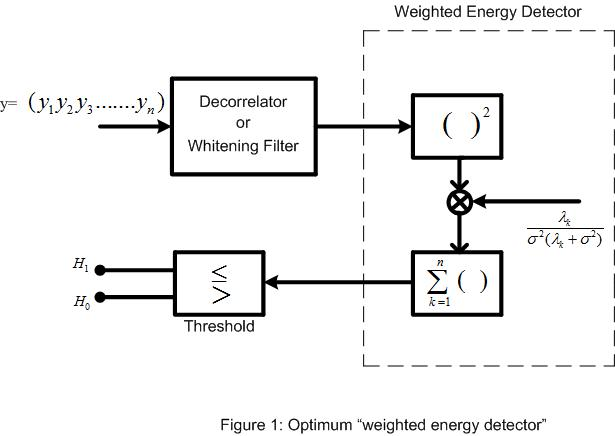
\includegraphics{figure1}\\
 \\
 \\
 \\
 \\\textbf{Interpretation 2: "Estimator - Correlator"}:\\
 The Quantity $\tilde{s}=\Sigma_s(\sigma^2I + \Sigma_s)^{-1}y$ is called a Wiener Filter. This is a very good estimator of the actual signal.\\
 Note: This quantity is also the minimum mean squared error estimator of S given Y=S+N.\\
 
 \ \ \ \ \ \ \ 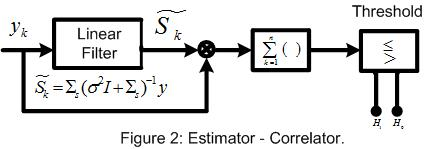
\includegraphics{figure2}.
 \section{Locally optimum detection of Stochastic Signals:}
 Consider a case, similar to a Composite Hypothesis Test:\\
 \begin{align*}
 \mathcal{H}_0 &: Y = N \in \mathbb{R}^n\\
 vs \\
 \mathcal{H}_1 &: Y = N+\sqrt{Q}S \in \mathbb{R}^n \ \ \ \ \ \ \ \ \ \ \ \ Q>0
 \end{align*}
 where,  
 \begin{align*}  
 N\sim \mathcal{N}(0,\sigma^2I)\\
 S\sim \mathcal{N}(0,\Sigma_s)
 \end{align*} \\
 The above situation can be looked as a case, where a signal is coming through a channel, which is blind to us, in terms of attenuation etc.\\
 \\For a fixed $Q>0$(i.e.,$\mathcal{H}_1$) vs Q=0(i.e.,$\mathcal{H}_0$) the detection statistic is\\ $y^TQ\Sigma_s(I+Q\Sigma_s)^{-1}y>\tau'$. As we see the statistic is dependent on Q.\\
 \\We see that in P($y:y^T\Sigma_s(I+Q\Sigma_s)^{-1}y>\tau') = \alpha$ is dependent on Q and hence no Universally Most Powerful(UMP) test exists(i.e., one single test does not exist) $\forall Q>0$.\\
\\ For finding the Locally most powerful test(LMP), let us consider the case of "Q=0" vs "Q$\neq$0(i.e., approximately Q=0).\\
For finding the LMP, we differentiate $y^T\Sigma_s(I+Q\Sigma_s)^{-1}y$ and set Q=0.\\
By doing so, we get the LMP test statistic as $2y^T\Sigma_sy$ and we use this quantity to compare with the threshold.\\
\\Consider a scaled version of the statistic ,\ \ \ \ \ \ $\frac{1}{n}y^T\Sigma_sy$.\\
Suppose $\Sigma_s$ is a matrix such that its (k,l)th element $\rho_{k,l}$ depends only on k-l. If such a condition occurs, this signal is said to be taken from a Wide Sense Stationary Process i.e., 
\begin{align*}
\rho_{k,l} \triangleq \rho_{k-l} \ \ \ \ \  i.e., Autocorrelation Function.
\end{align*}.\\
\\Using the above Wide Sense Stationary structure to the white noise that we earlier considered , we can write
\begin{equation*}
\begin{aligned}
T(y)&=\frac{1}{n}y^T\Sigma_sy \\
&=\frac{1}{n}\Sigma_{k=1}^{n}\Sigma_{l=1}^{n}y_ky_l\rho_{k-l} \\
&=\rho_0\hat{\rho_0} + 2\Sigma_{k=1}^{n-1}\rho_k\hat{\rho_k}.
\end{aligned}
\end{equation*}\\
where, $\hat{\rho_k}\colon=\frac{1}{n-k}\Sigma_{l=1}^{n-k}y_ly_{l+k}$ \ \ \ \ \ \ \ $\forall k \in [n]$, which the sample estimate of correlation at lag k.\\
For $n\gg k, \hat{\rho_k}$ turns out to be a good estimate of $E[Y_l Y_{l+k}]$.\\
\\From the above equations, we can see that T(Y) estimates the cross covariance structure of the signal y and correlates it with signal covariance $(\rho_k)_{k=1}^{n}$.\\
\\Roughly, if $\hat{\rho_k}$ is "accurate", then:\\
\begin{equation*}
T(y)=
\begin{cases}
 1 , under H_0\\
 \rho_0+Q(\rho_0^2+2\Sigma_{k=1}^{n-1}\rho_k^2), under H_1.
\end{cases}
\end{equation*}\\
where \ \ \ \ \ \ \ \ \ \ \ \ \ \ \ \  $\hat{\rho_k}= E[Y_l Y_{l+k}]$.\\
Since we are dealing with Autocorrelation functions and could end up getting equations which involve Convolutions, we choose an intelligent method of going to the frequency domain, by taking the Fourier Transform of the Autocorrelation function which gives us the Power Spectral density(P.S.D).\\
\begin{equation*}
T(y)=\frac{1}{2\pi}\int_{-\infty}^{\infty}\phi(\omega)\hat{\phi(\omega)}d\omega
\end{equation*}\\
where $\phi(\omega)$  is the P.S.D of S(signal) at $\omega$.\\
and,
\begin{equation*} \hat{\phi(\omega)}=\frac{1}{n}|\Sigma_{k=1}^{n}y_ke^{j\omega k}|^2.
\end{equation*}\\
This computes the spectrum of our signal and correlates with the spectrum of the desired signal.

\end{document}